% Kopfzeile beim Kapitelanfang:
\fancypagestyle{plain}{
%Kopfzeile links bzw. innen
\fancyhead[L]{\Large Vorlesung 27 (27.01.2013)}
%Kopfzeile rechts bzw. außen
\fancyhead[R]{}}
%Kopfzeile links bzw. innen
\fancyhead[L]{\Large Vorlesung 27 (27.01.2014)}
%Kopfzeile rechts bzw. außen
\fancyhead[R]{}
% **************************************************
\subsection*{Merkregel}
$x=\varphi(t) \Ra dx = \varphi'(t) dt +$ Grenzen substituieren\nl
In Praxis oft: $\varphi$ streng monoton ($\Ra$ bijektiv). Dann:
$$\int_c^d f(x) dx = \int_{\varphi^{-1}(c)}^{\varphi^{-1}(d)} f(\varphi(t)) \cdot \varphi'(t) dt$$

\subsection*{Beweis}
Sei $F$ Stammfunktion von $f$\\
$\Ra (F \circ \varphi)'(t) \underset{Kettenregel}{=} \underbrace{F'}_{f}(\varphi(t)) \cdot \varphi'(t)$\\
$\underset{\text{HDI (\ref{14.11})}}{\Ra} \int_a^b f(\varphi(t)) \cdot \varphi'(t) dt = (F \circ \varphi) \arrowvert_a^b = F(\varphi(b)) - F(\varphi(a)) \underset{\text{HDI (\ref{14.11})}}{=} \int_{\varphi(a)}^{\varphi(b)} f(x) dx$ \qed

\subsection*{Beispiele}
\enk{
\item $c \in \R \setminus \{0\} \Ra \int_a^b f(ct) dt \underset{\begin{array}{l} x=ct \\ dx = c \cdot dt \end{array}}{=} \frac{1}{c} \int_{ca}^{cb} f(x) dx$
\item $\int_a^b f(t+c) dt \underset{\begin{array}{l} x=t+c \\ dx = dt \end{array}}{=} \int_{a+c}^{b+c} f(x) dx$
\newpage
\item \underline{Fläche des Einheitskreises} (Radius 1)\nl
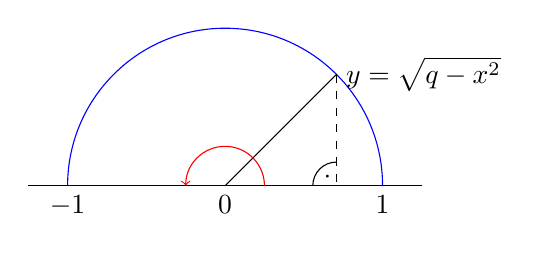
\begin{tikzpicture}
\draw (-2.5,0)--(2.5,0); 
\draw[color=blue](2,0) arc (0:180:2);
\draw (-2,0) node[below] {$-1$} (2,0) node[below] {$1$} (0,0) node[below] {$0$};
\draw (0,0)--(1.41421356,1.41421356) node[right] {$y=\sqrt{q-x^2}$};
\draw[dashed] (1.41421356,1.41421356)--(1.41421356,0);
\draw (1.41421356,0.3) arc (90:180:0.3);
\draw (1.3,0.1) node {$\cdot$};
\draw[color=red,->] (0.5,0) arc (0:180:0.5);
\end{tikzpicture}\nl
$F=2 \cdot \int_{-1}^1 \sqrt{1-x^2} dx = ?$\nl
\begin{tikzpicture}
\draw (-0.5,0)--(3.5,0);
\draw (0,-1.5)--(0,1.5);
\draw[color=blue,domain=0:3.14159265] plot (\x, {cos(deg(\x))});
\draw[dashed] (3.14159265,-1)--(3.14159265,0) node[above] {$\pi$};
\end{tikzpicture}\nl
Substituiere: $x=\underbrace{\cos(t)}_{\text{streng mon. auf } [0,\pi]}=\varphi(t), dx=-\sin(t) dt, t \in [0,\pi]$\\
$\Ra \int_{-1}^1 \sqrt{1-x^2} dx = - \int_{-1}^1 \sqrt{1-\cos^2(t)} \sin(t) dt = \int_0^\pi sin^2(t) dt$\\
$\underline{\int \sin^2(t) dt} = \underset{f}{\int \sin(t)} \cdot \underset{g'}{\sin(t)} dt \underset{\text{part. Int.}}{=} -\sin(t) \cdot \cos(t) + \underbrace{\int \cos^2(t) dt}_{=t-\underline{\int \sin^2(t) dt}}$\\
$\Ra \int \sin^2(t) dt = \frac{1}{2}(t-\sin(t) \cdot \cos(t))$\\
$\Ra f=(t-\sin(t) \cdot \cos(t)) \arrowvert_0^\pi = \underline{\underline{\pi}}$
\item $\underbrace{\int_a^b \frac{\varphi'(t)}{\varphi(t)}}_{=\int_{\varphi(a)}^{\varphi(b)} \frac{dx}{x} - \ln|x| \arrowvert_{\varphi(a)}^{\varphi(b)} = \ln \left|\frac{\varphi(b)}{\varphi(a)}\right|}$, dabei $\varphi: [a,b] \to \R$ stetig differenzierbar und nullstellenfrei
}

\subsection*{Bemerkung}
$\int x^n \sin(x) dx, \int x^n e^x dx,$ etc.\\
Sukzessives Verkleinern des Exponenten $n$ durch partielles Integrieren

\subsubsection*{Beispiel}
$\int \underset{f}{x^n} \underset{g'}{e^x} dx = x^n e^x - n \cdot \int x^{n-1} e^x = \ldots$

\subsection*{Vorsicht}
Oft gibt es zu selbst zu einfachen Integranden keine geschlossen angebbare Stammfunktion!

\subsubsection*{Beispiele}
$\int e^{-x^2} dx$, $erf(x) := \int_0^x e^{-t^2} dt$ Gaußsche Fehlerfunktion, $\int \frac{\sin(x)}{x} dx$

\phantomsection
\addcontentsline{toc}{chapter}{Uneigentliche Integrale}
\chapter*{Uneigentliche Integrale}\label{UneigentlicheIntegrale}
\underline{Bisher}: Integration von Regelfunktionen über kompakte Intervalle\nl
\underline{Jetzt}: Ausdehnung auf allgemeine Intervalle, unbeschränkte Integranden

\subsection*{Beispiel}
$\int_0^1 \frac{dx}{x^2}=?$\\
$0$ ist hier die kritische Grenze: $\frac{1}{x^2}$ ist in $0$ nicht definiert!\nl
Betrachte $\int_\alpha^1 \frac{dx}{x^2}$ mit $\alpha \downarrow 0$. Existiert der Limes?\nl
Alternativ: $\int_1^\infty \frac{dx}{x^2}=?$\nl

\begin{tikzpicture}
\draw[color=white,pattern=custom north west lines,hatchcolor=blue] (0,0) -- (0,2.5) -- (0.63244555,2.5) -- plot [domain=0.63244555:1] (\x, {1/(\x^2)}) -- (1,0) -- cycle;
\draw[color=white,pattern=custom north west lines,hatchcolor=red] (1,0) -- plot [domain=1:3.5] (\x, {1/(\x^2)}) -- (3.5,0) -- cycle;
\draw[->] (-0.5,0)--(3.5,0);
\draw[->] (0,-0.5)--(0,2.5);
\draw[color=blue,domain=0.6324555:3.5] plot (\x, {1/(\x^2)});
\draw (1,1)--(1,0) node[below] {$1$} (1,1)--(0,1) node[left] {$1$};
\draw[color=blue] (0.5,0.5)--(2,2) node[right] {$\int_0^1 \frac{1}{x^2} dx$};
\draw[color=red] (2,0.125)--(2,1) node[right] {$\int_1^\infty \frac{1}{x^2} dx$};
\end{tikzpicture}

\subsection*{Bezeichnung}
Sei $I \subseteq \R$ beliebiges Intervall.\\
$f: I \to \R$ heißt \underline{Regelfunktion} $:\Lra$\\
$f \arrowvert_[a,b]$ Regelfunktion $\forall$ kompakten $[a,b] \subseteq I$

\section{Definition}\label{14.15}
\en{
\item Sei $f: (a,b] \to \R$ Regelfunktion, $-\infty \le a < b < \infty$:\\
$\int_a^b f(x) dx := \lim_{\alpha \downarrow a} \int_\alpha^b f(x) dx$ sofern der Limes existiert.\\
Man sagt dann: Das uneigentliche Integral von $f$ über $(a,b]$ existiert/konvergiert.
\item $f: [a,b) \to \R$ Regelfunktion, $-\infty < a < b \le \infty$:\\
$\int_a^b f(x) dx := \lim_{\beta \uparrow b} \int_a^\beta f(x) dx$ sofern der Limes existiert.
\item $f: (a,b) \to \R$ Regelfunktion, $-\infty \le a < b \le \infty$:\\
Wähle $c \in (a,b)$ und setze $\int_a^b f(x) dx := \int_a^c f(x) dx + \int_c^b f(x) dx$, sofern \underline{beide} uneigentlichen Integrale existieren!\\
\emph{(Diese Definition ist unabhängig von der Wahl von $c$)}
}

\newpage

\section{Beispiele}\label{14.16}
\en{
\item $\int_0^\infty e^{-ax} dx, a \in \R$, kritisch: $\infty$
\enk{
\item $a \le 0: \beta > 0 \Ra \int_0^\beta e^{-ax} dx \ge \int_0^\beta 1 dx = \beta \Ra \int_0^\infty e^{-ax} dx$ divergiert
\item $a > 0: \int_0^\beta e^{-ax} dx = -\frac{1}{a} e^{-ax} \arrowvert_0^\beta = \frac{1}{a}(1-e^{-a\beta}) \underset{\beta \to \infty}{\to} \frac{1}{a}$
}
\item $\int_1^\infty \frac{dx}{x^s}$ ($s \in \R$), $x^s=e^{s \cdot \ln(x)}$ ($x > 0$), kritisch: $\infty$\\
$\beta > 1 \Ra \int_1^\beta \frac{dx}{x^s} = \left\{\begin{array}{l l} \frac{1}{-s+1} x^{-s+1} \arrowvert_1^\beta = \frac{1}{s-1}(1-\frac{1}{\beta^{s-1}}), & s \neq 1 \\ \underbrace{\ln(x) \arrowvert_1^\beta}_{\ln(\beta)}, & s=1 \end{array} \right.$\\
$\beta \to \infty \Ra \int_1^\infty \frac{dx}{x^s} = \left\{\begin{array}{l l} \frac{1}{s-1}, & s>1 \\ \text{divergiert}, & s \le 1 \end{array} \right.$\nl
Insbes.: $\int_1^\infty \frac{dx}{x^2} = 1$
\item $\int_0^1 \frac{dx}{x^2}$, kritisch: $0$ (falls $s>0$)\\
$0 < \alpha < 1 \Ra \int_\alpha^1 \frac{dx}{x^s} \underset{\text{s.o.}}{=} \left\{\begin{array}{l l} \frac{1}{1-s} (1-\alpha^{1-s}), & s \neq 1 \\ -\ln(\alpha), & s=1 \end{array} \right.$\\
$\alpha \downarrow 0 \Ra \int_0^1 \frac{dx}{x^s} = \left\{\begin{array}{l l} \frac{1}{1-s}, & s<1 \\ \text{divergiert}, & s \ge 1 \end{array}\right.$
\item Beispiel zur Vorsicht: $\int_{-\infty}^\infty x dx = ?$\\
$\lim_{R \to \infty} \int_{-R}^R x dx = \lim_{R \to \infty} \frac{x^2}{2} \arrowvert_{-R}^R = 0$\\
Aber: $\int_{-\infty}^\infty x dx$ existiert nicht, da die Limiten $+\infty, -\infty$ getrennt zu nehmen sind, und $\int_0^\infty x dx$ divergiert.
}
Wichtiges Kriterium für die Konvergenz uneigentlicher Integrale:

\newpage

\section{Majorantenkriterium}\label{14.17}
Seien $f,g: [a,b) \to \R$ Regelfunktionen mit $g \ge 0$ und $|f| \le g$.\\
Angenommen, $\int_a^b g(x) dx$ existiert $\Ra \int_a^b f(x) dx$ existiert.\nl
Entsprechend für $(a,b], (a,b)$

\subsection*{Beweis}
Der Beweis basiert auf dem \underline{Cauchy-Kriterium für Grenzwerte} (\ref{5.15}):\\
Sei $h: [a,b) \to \R$ eine Funktion. Dann gilt: $\exists \lim_{x \uparrow b} h(x) :\Lra \forall \eps > 0 \exists s \in [a,b): |h(x)-h(y)| < \eps \forall x,y \in [s,b)$\nl
%TODO: Grafik (3) (vielleicht noch aus fremder Mitschrift abtexen?)
\underline{Beweis des Majorantenkriteriums}: $F(x) := \int_a^x f(t) dt, G(x) := \int_a^x g(t) dt, x \in [a,b)$\\
$x \le < \Ra |F(y)-F(x)| \le \int_x^y |f(t)| dt \underset{\text{vor.}}{\le} \int_x^y g(t) dt = G(y)-G(x)$ (*)\nl
$\exists \lim_{x \uparrow b} G(x) \Ra G$ erfüllt Cauchy-Bedingung in der kritischen Obergrenze $b$ (s.o.)\\
$\underset{\text{(*)}}{\Ra}$ auch $F$ erfüllt Cauchy-Bedingung in $b \Ra \exists \lim_{x \uparrow b} F(x)$ \qed

\section{Grenzwertkriterium}\label{14.18}
Seien $f,g: [a,b) \to \R$ Regelfunktionen, $g > 0$\\
Angenommen, $\exists \int_a^b g(x) dx$ \underline{und} $\exists \lim_{x \uparrow b} \frac{f(x)}{g(x)} =: c \in \R \Ra \exists \int_a^b f(x) dx$

\subsection*{Beweis}
Vorauss. $\Ra \exists s \in [a,b): \left|\frac{f(x)}{g(x)}\right| \le |c|+1 \forall x \in [s,b)$\\
d.h. $|f(x)| \le (|c|+1) \cdot g(x)$ auf $[s,b)$\\
Majorantenkrit. $\Ra$ Beh. \qed